\documentclass[aspectratio=169]{beamer}

\usetheme{default}
\usecolortheme{default}
\setbeamertemplate{navigation symbols}{}
\setbeamertemplate{footline}[frame number]

\usepackage[T1]{fontenc}
\usepackage{lmodern}
\usepackage{graphicx}
\usepackage{booktabs}
\usepackage{array}
\usepackage{amsmath}

\graphicspath{{../results/}}

\title{CLEVR Set Prediction Ablations}
\subtitle{Final Package, Failure Modes, and Benchmark Next Steps}
\author{}
\date{\today}

\begin{document}

\begin{frame}
  \titlepage
\end{frame}

\begin{frame}{Setup and Protocol}
\small
\begin{itemize}
  \item Current task in this study: noisy CLEVR state set $\rightarrow$ clean CLEVR state set.
  \item Main metric: validation Hungarian-matched distance (`val\_matched\_dist`), lower is better.
  \item Standard fast-study configuration:
  \begin{itemize}
    \item batch size 512, lr auto-scaled from $3\times10^{-4}$ at batch 64
    \item up to 200 epochs, with some runs using early stopping and some rerun without it
    \item 70k train scenes with capped validation for rapid iteration
  \end{itemize}
  \item Every result below was re-checked from the saved `.pkl` artifacts and regenerated plots.
\end{itemize}
\end{frame}

\begin{frame}{Executive Summary}
\small
\begin{tabular}{>{\raggedright\arraybackslash}p{5.0cm} >{\raggedright\arraybackslash}p{5.1cm} >{\raggedleft\arraybackslash}p{1.8cm}}
\toprule
Question & Checked answer & Best dist \\
\midrule
Default full-data winner & PM3 $\tau=0.12$ beats Hungarian and Chamfer & 0.7010 \\
Best single-factor PM3 gain & warmup\_cosine schedule & 0.5495 \\
Best PM3 grid point & $\tau=0.12$ + warmup + standard decoder & 0.5828 \\
Did early stopping hurt PM3 best recipe? & Yes: 0.7039 $\rightarrow$ 0.6607 without early stop & 0.6607 \\
Best combined-recipe model overall & Hungarian + slots + warmup\_cosine & 0.4314 \\
\bottomrule
\end{tabular}

\vspace{0.6em}
\footnotesize
\begin{itemize}
  \item The strong PM3 ingredients are real, but they do not add linearly.
  \item The biggest surprise is that the combined recipe helps Hungarian far more than PM3.
\end{itemize}
\end{frame}

\begin{frame}{Single-Factor PM3 Wins}
\small
\begin{tabular}{>{\raggedright\arraybackslash}p{4.0cm} >{\raggedright\arraybackslash}p{4.3cm} >{\raggedleft\arraybackslash}p{1.6cm} >{\raggedleft\arraybackslash}p{1.4cm}}
\toprule
Study & Best run & Best dist & Epoch \\
\midrule
Temperature sweep & $\tau=0.15$ & 0.5625 & 177 \\
Learning-rate schedule & warmup\_cosine & 0.5495 & 187 \\
Slot embeddings & PM3 (slotted) & 0.6094 & 190 \\
Baseline comparison & PM3 $\tau=0.12$ & 0.7010 & 176 \\
Power sweep & $p=3.0$ & 0.7010 & 176 \\
\bottomrule
\end{tabular}

\vspace{0.6em}
\footnotesize
\begin{itemize}
  \item Each ingredient looks individually helpful for PM3.
  \item That made the combined-recipe regression non-obvious and worth isolating.
\end{itemize}
\end{frame}

\begin{frame}{Temperature Sweep}
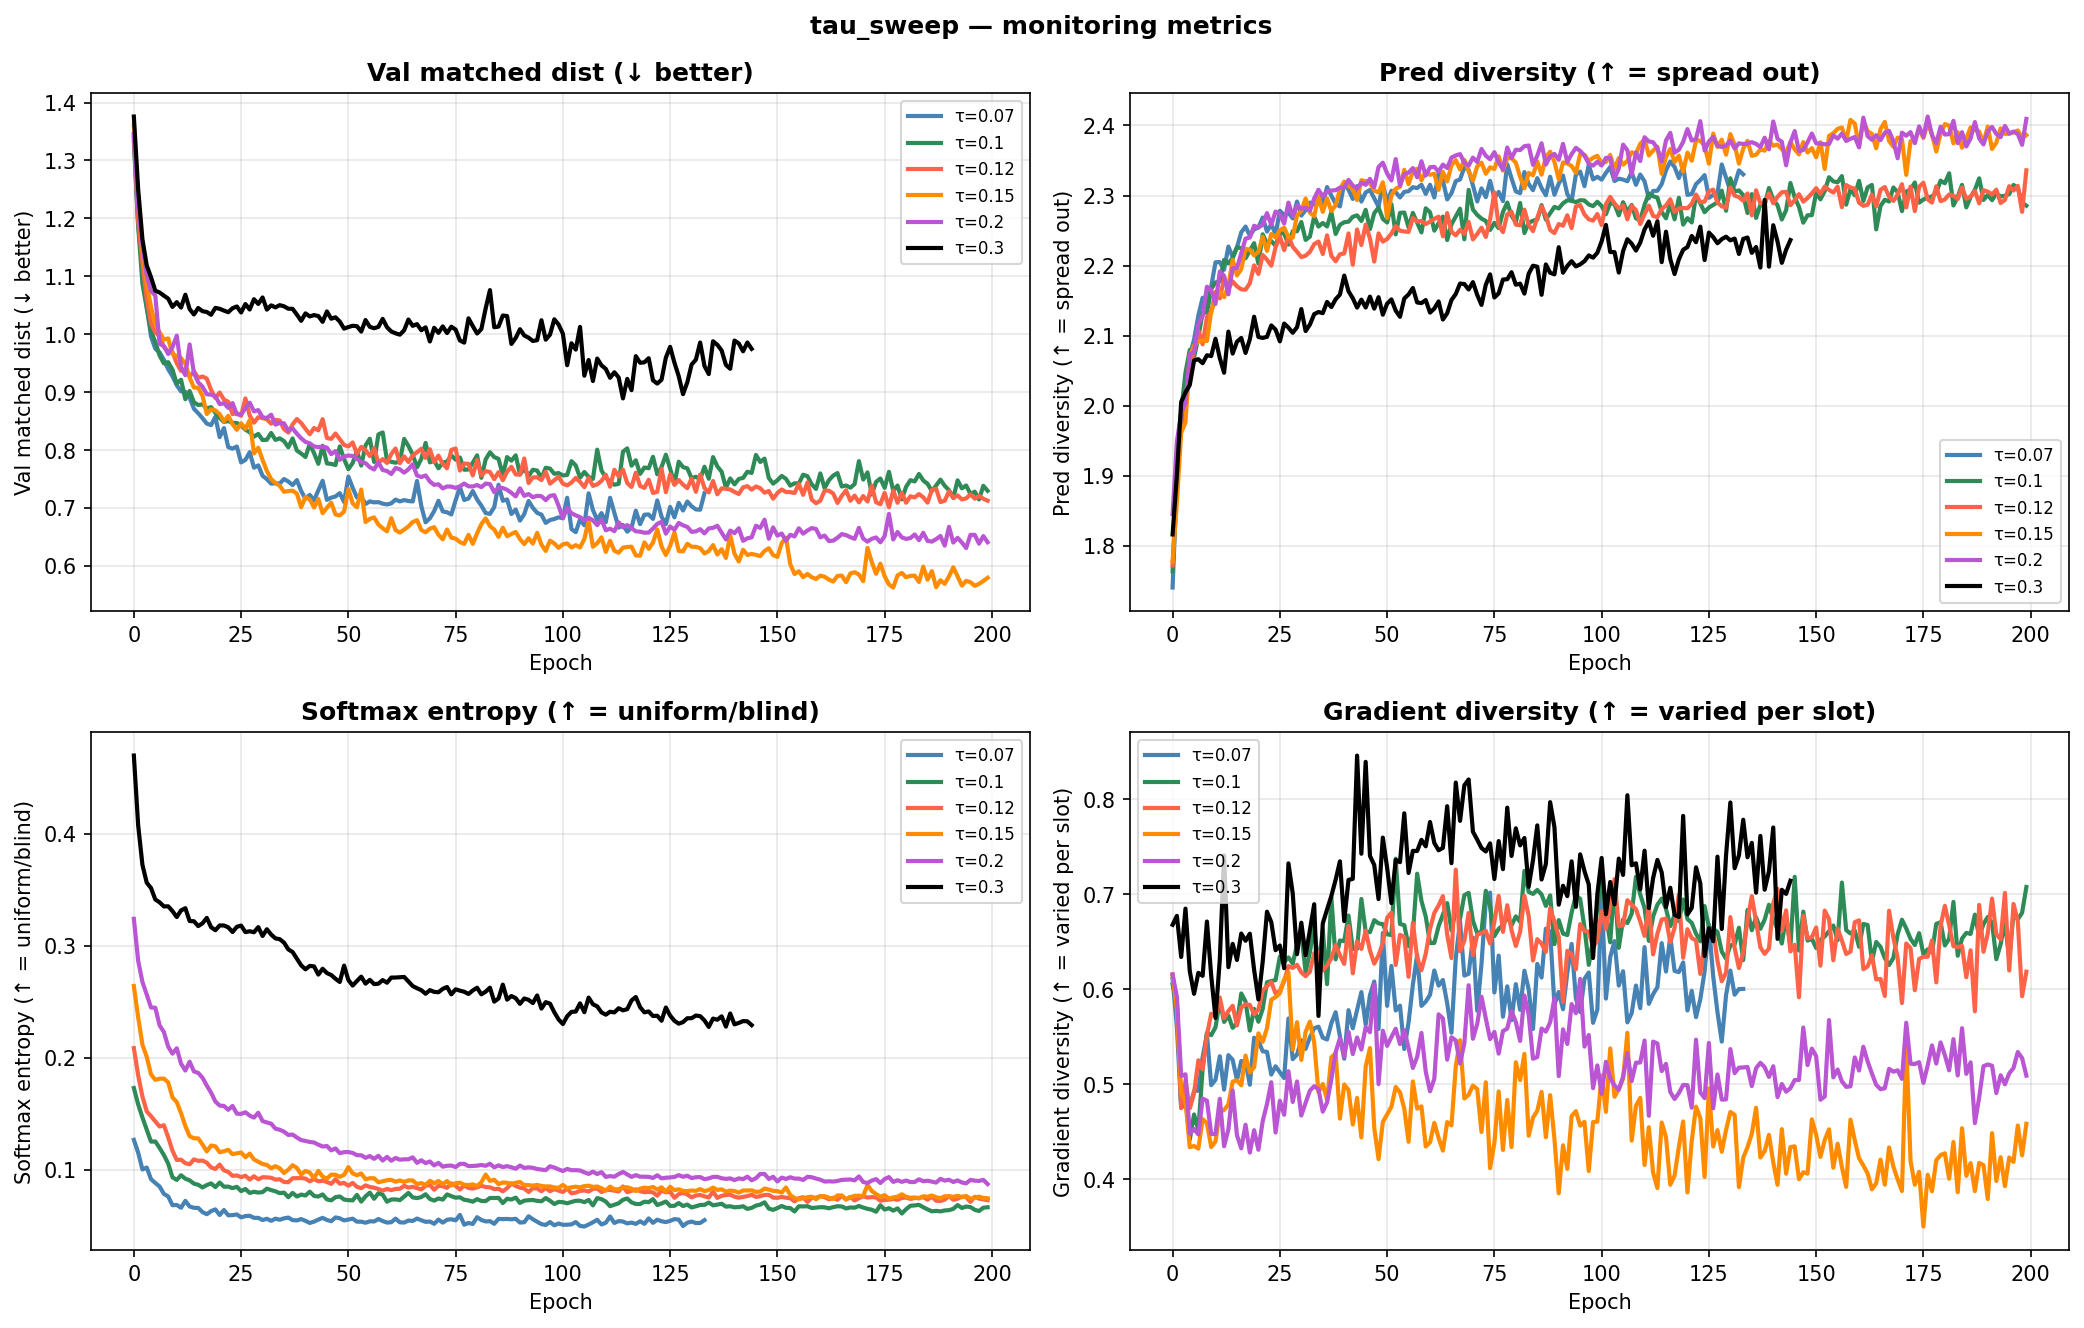
\includegraphics[width=\textwidth,height=0.63\textheight,keepaspectratio]{tau_sweep_monitoring.png}

\vspace{0.3em}
\footnotesize
\begin{itemize}
  \item Best run: $\tau=0.15$, best dist $0.5625$ at epoch 177, final $0.5794$.
  \item $\tau=0.20$ is next best at $0.6307$; $\tau=0.30$ degrades sharply to $0.8891$.
  \item Very small $\tau$ values recover coverage more slowly and plateau higher than $\tau=0.15$.
\end{itemize}
\end{frame}

\begin{frame}{Learning-Rate Schedule}
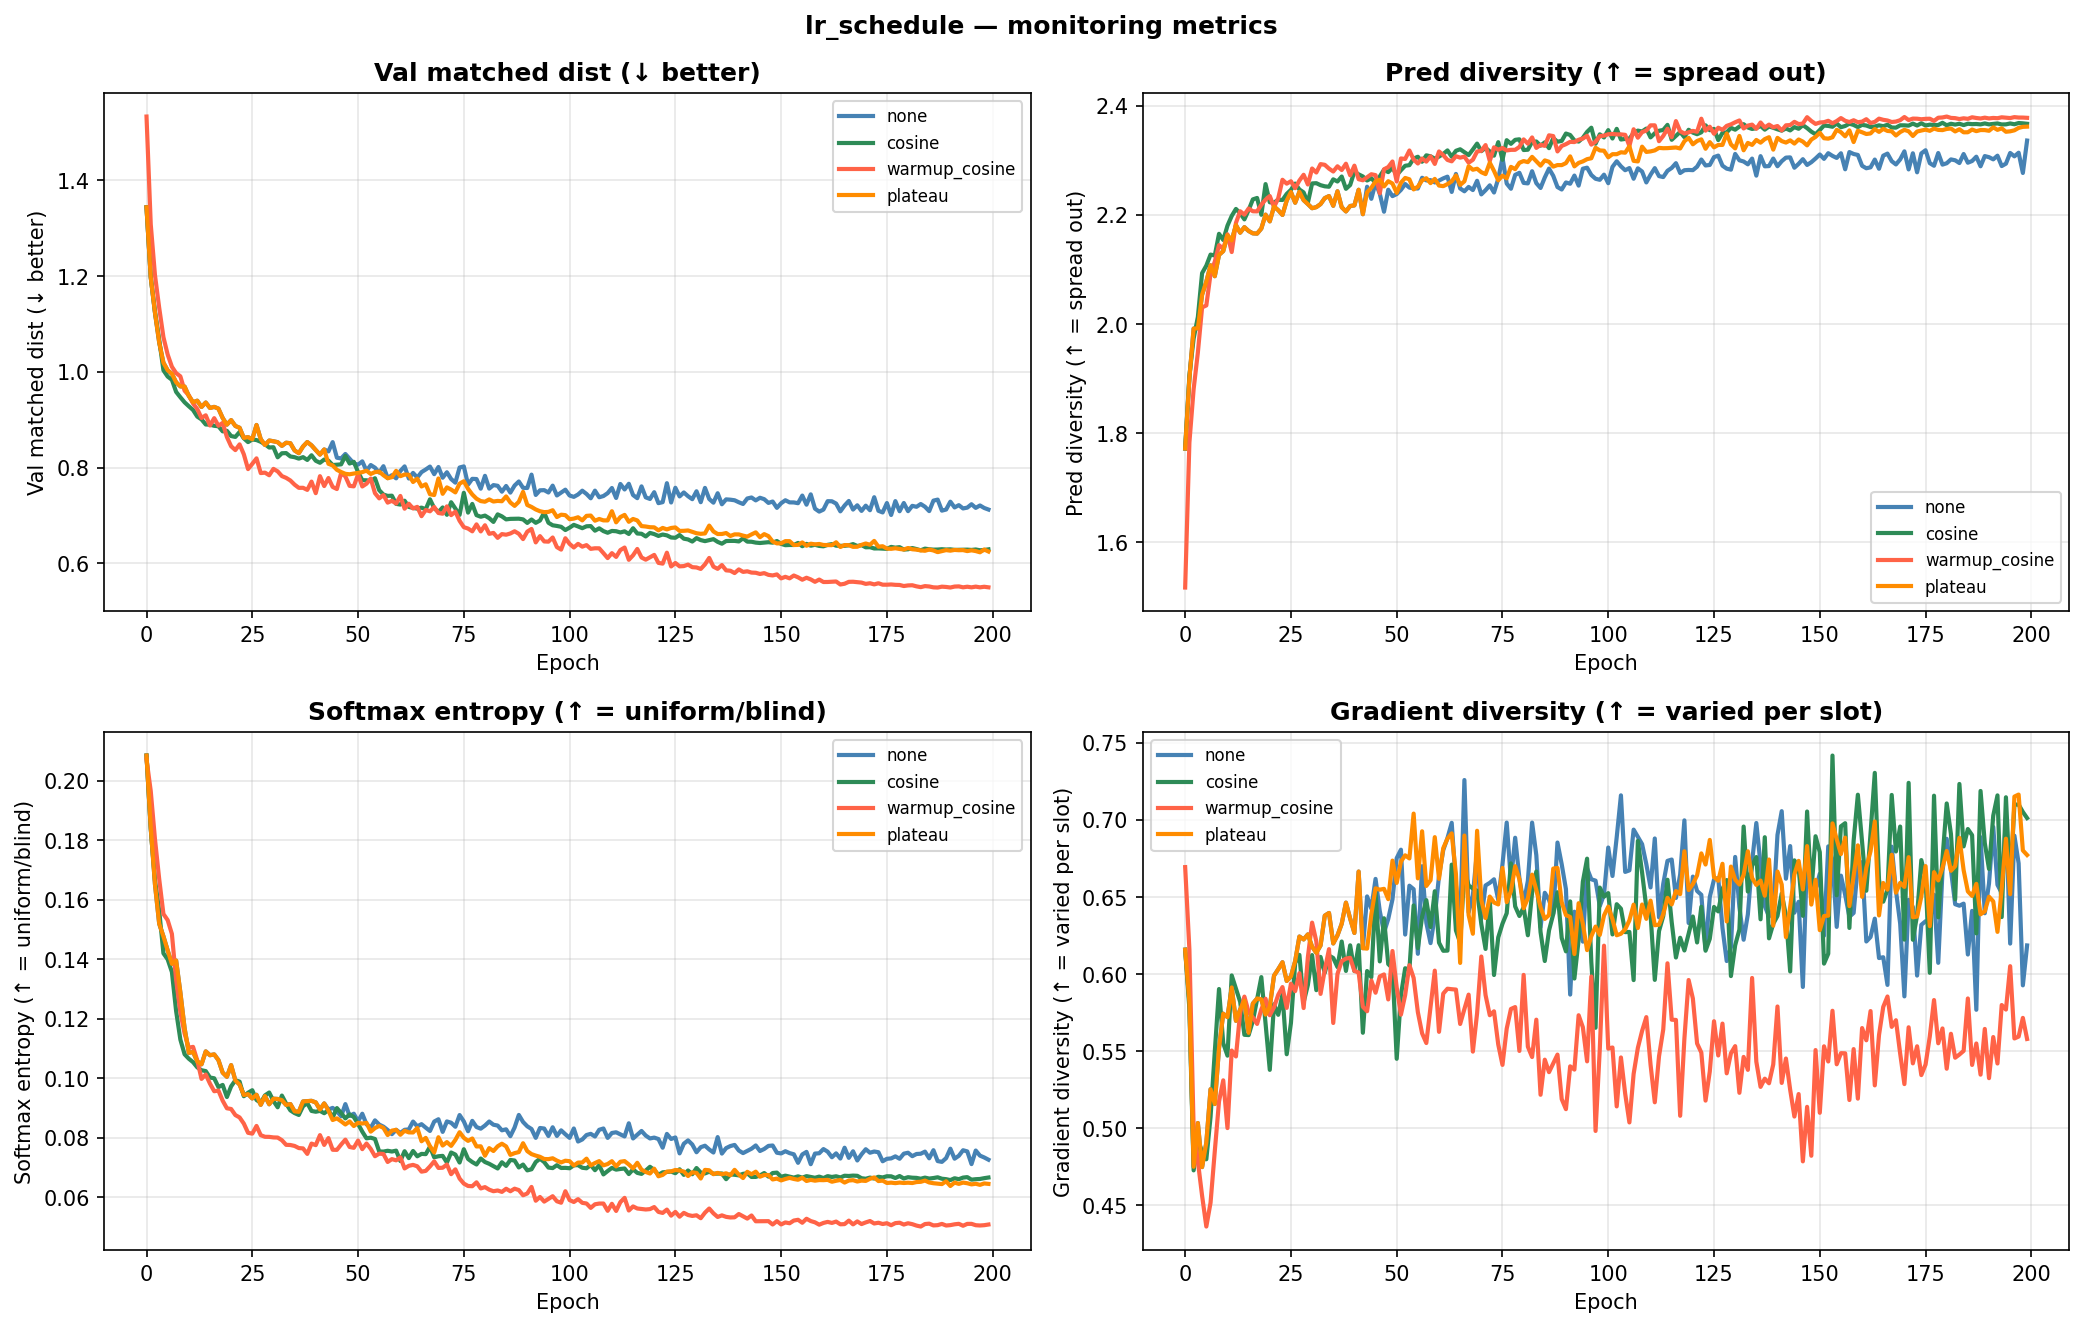
\includegraphics[width=\textwidth,height=0.63\textheight,keepaspectratio]{lr_schedule_monitoring.png}

\vspace{0.3em}
\footnotesize
\begin{itemize}
  \item warmup\_cosine gives the strongest PM3 run: best dist $0.5495$, final $0.5499$.
  \item plateau and cosine also help materially ($0.6231$ and $0.6273$).
  \item Leaving the lr fixed stalls at the default PM3 level ($0.7010$).
\end{itemize}
\end{frame}

\begin{frame}{Default Baseline Comparison}
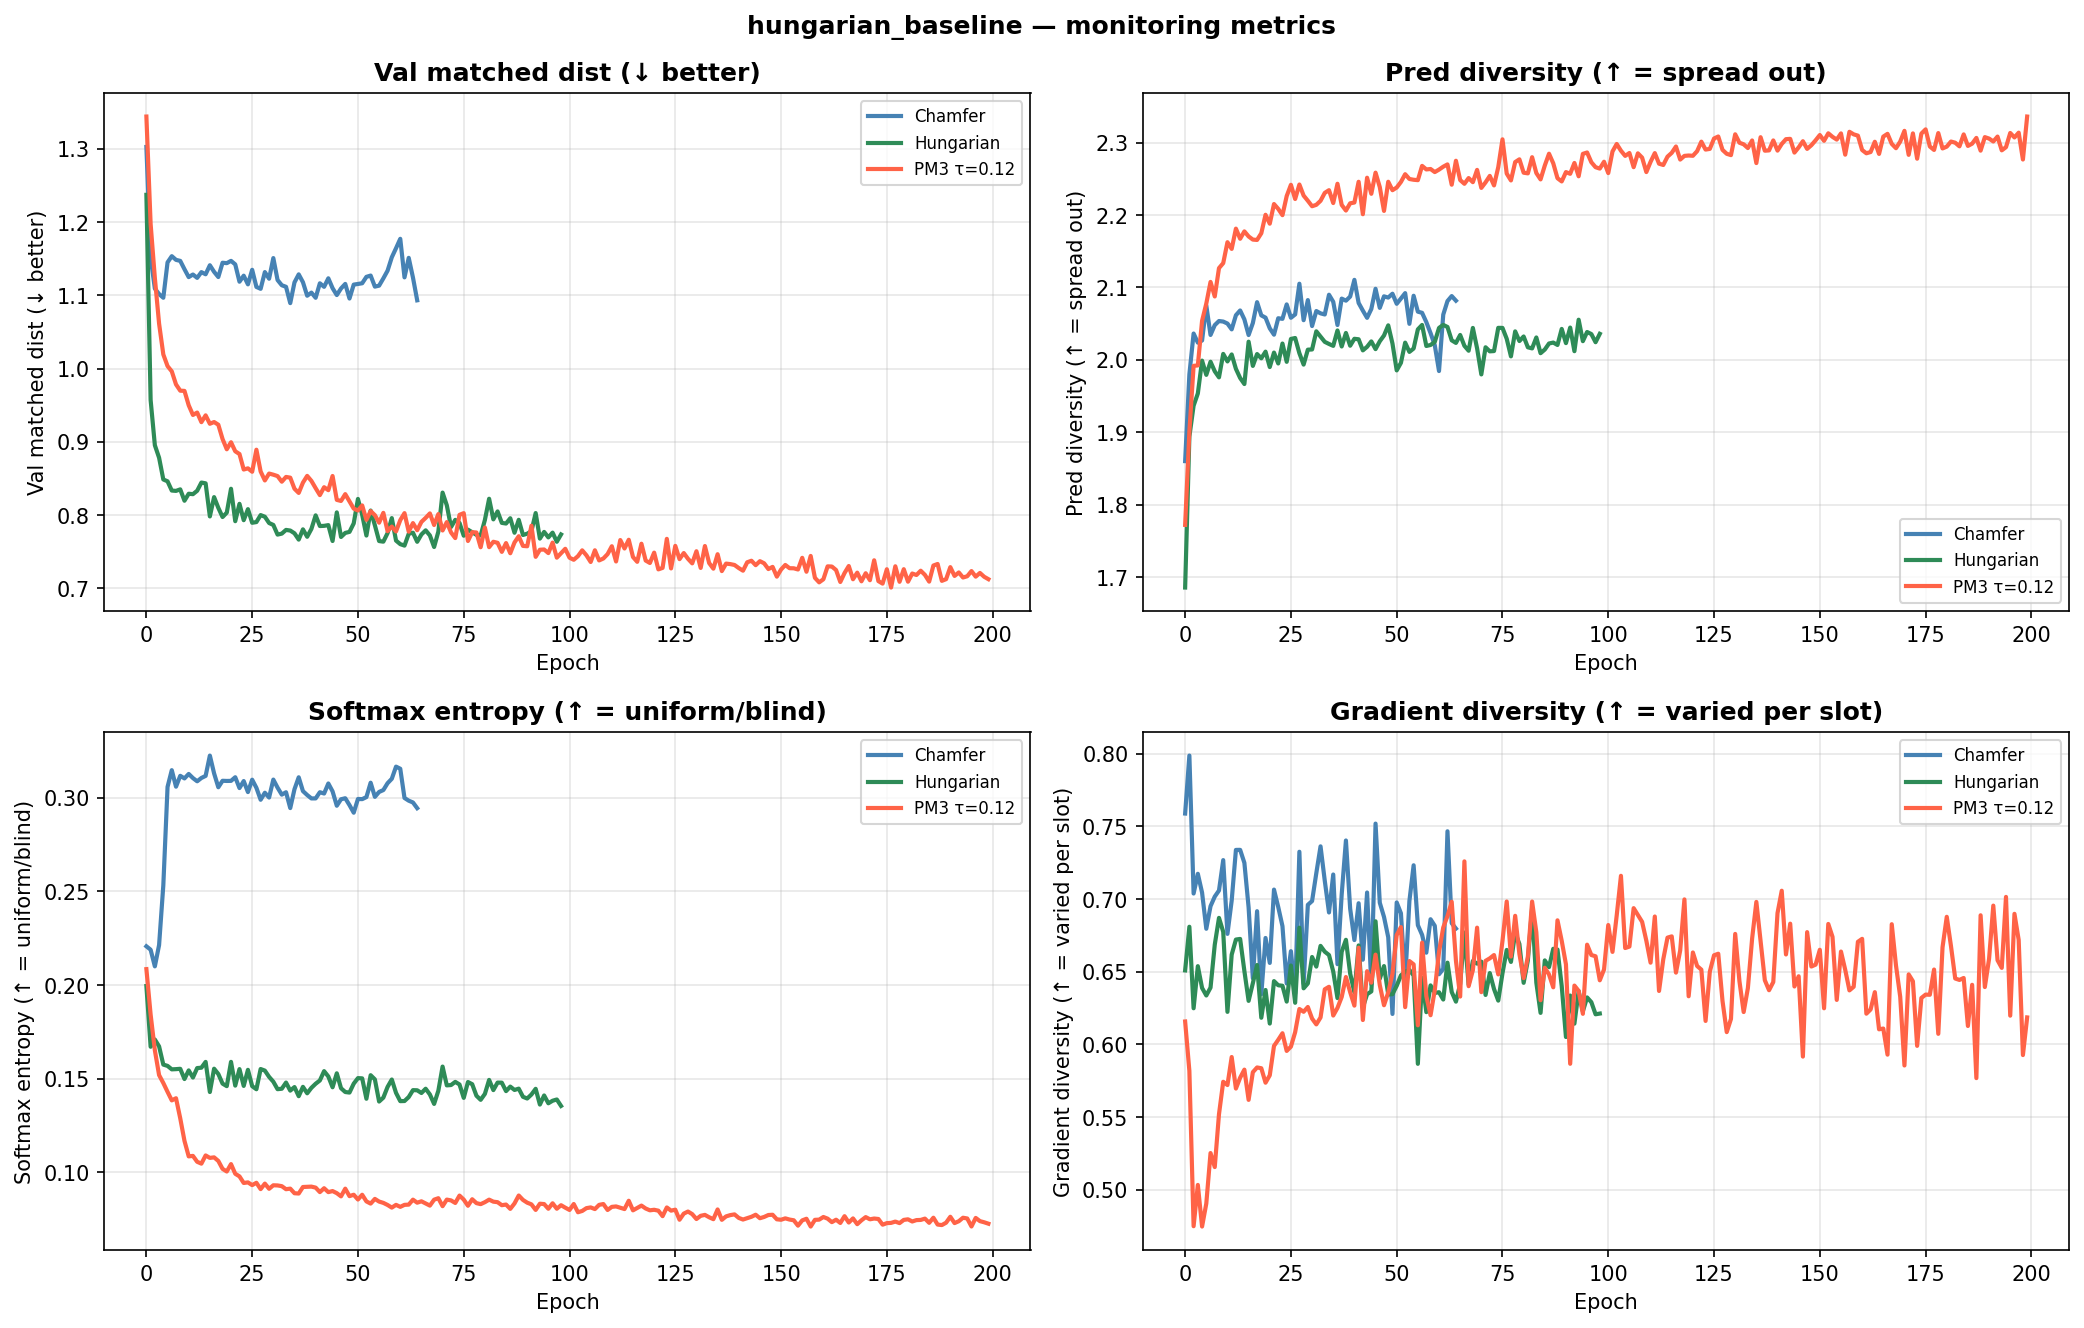
\includegraphics[width=\textwidth,height=0.63\textheight,keepaspectratio]{hungarian_baseline_monitoring.png}

\vspace{0.3em}
\footnotesize
\begin{itemize}
  \item Under the default full-data recipe, PM3 wins: $0.7010$ vs Hungarian $0.7564$ vs Chamfer $1.0893$.
  \item Hungarian is clearly stronger than Chamfer, but still behind PM3 on the matched-distance metric.
  \item This is the baseline result that motivated the recipe search.
\end{itemize}
\end{frame}

\begin{frame}{Combined Recipe: Apples-to-Apples Surprise}
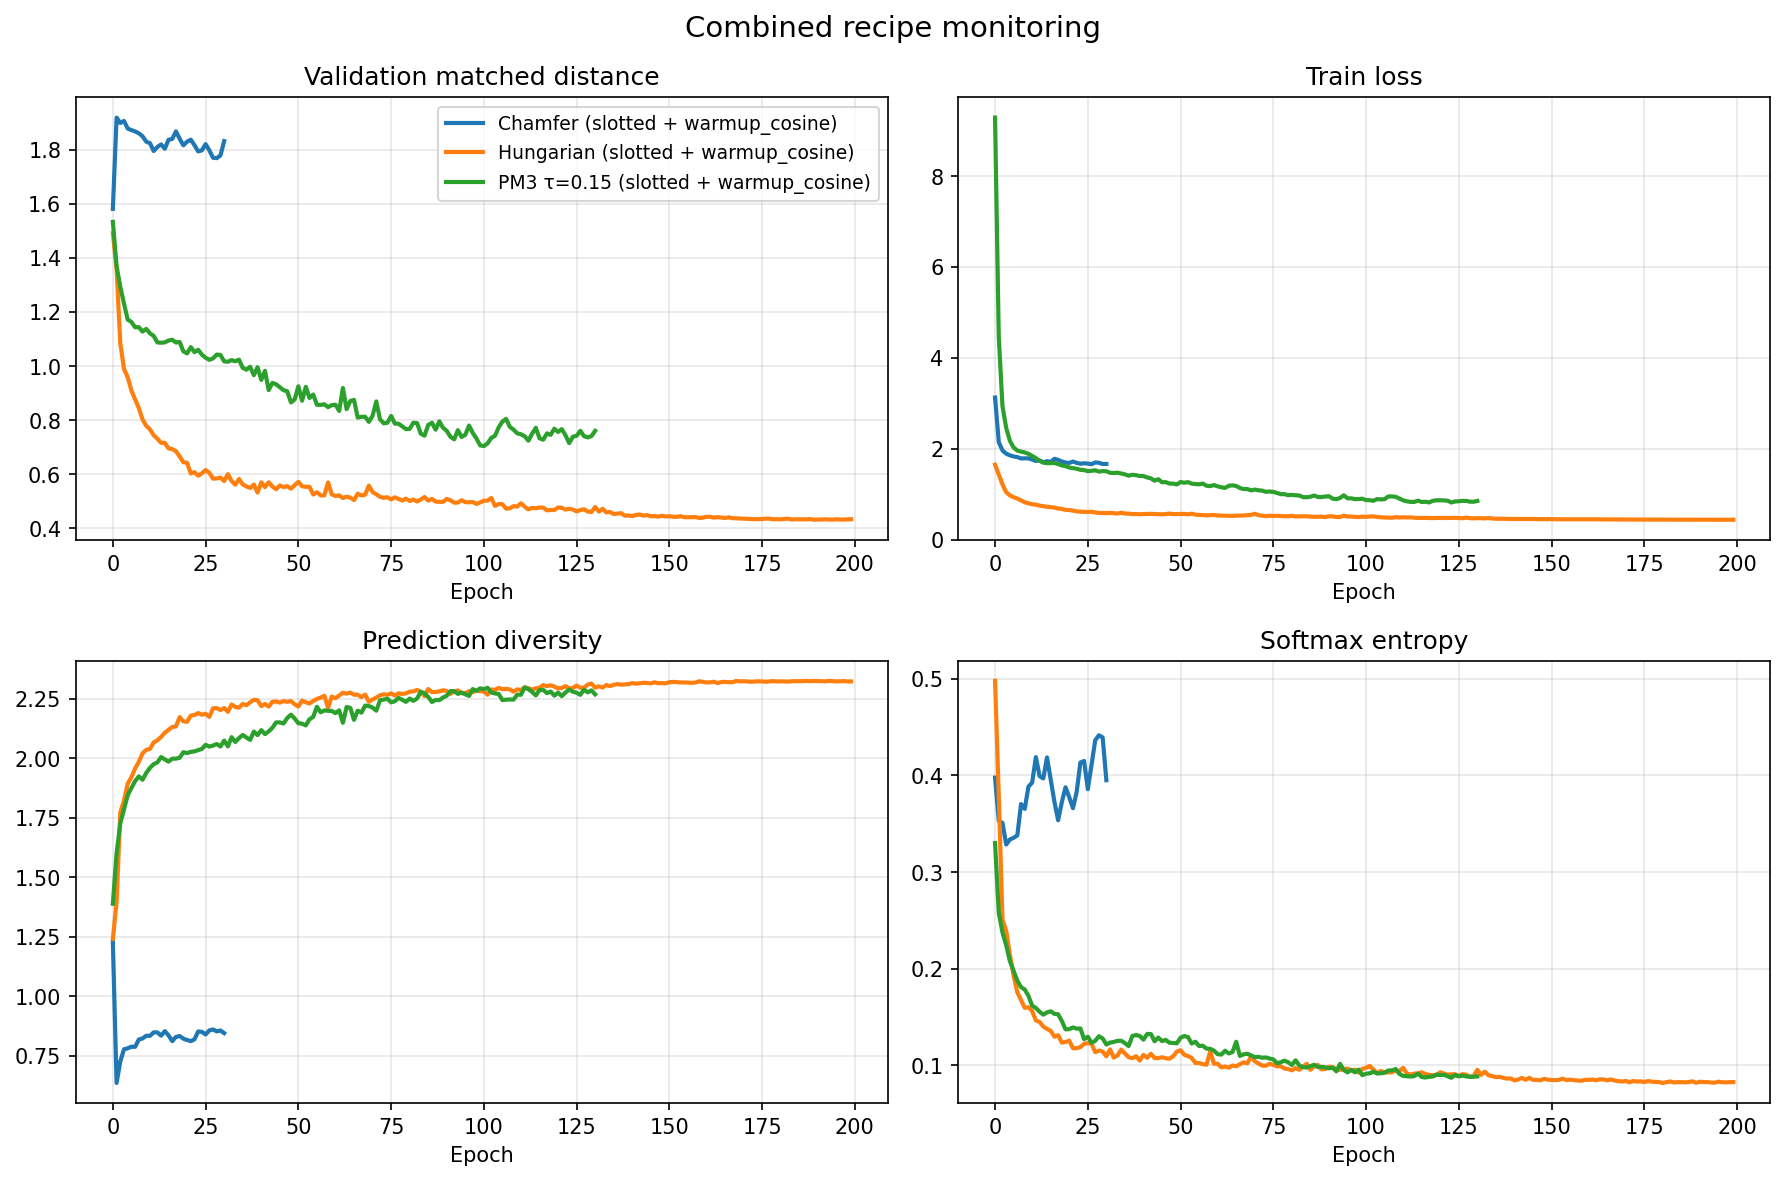
\includegraphics[width=\textwidth,height=0.63\textheight,keepaspectratio]{combined_recipe_monitoring.png}

\vspace{0.3em}
\footnotesize
\begin{itemize}
  \item Combined recipe = slotted decoder + warmup\_cosine for all losses, PM3 at $\tau=0.15$.
  \item Hungarian becomes the clear winner: best dist $0.4314$, final $0.4331$.
  \item PM3 under the same recipe is much worse: best $0.7039$ before early stopping; Chamfer fails badly from epoch 0.
\end{itemize}
\end{frame}

\begin{frame}{PM3 Best Recipe Without Early Stopping}
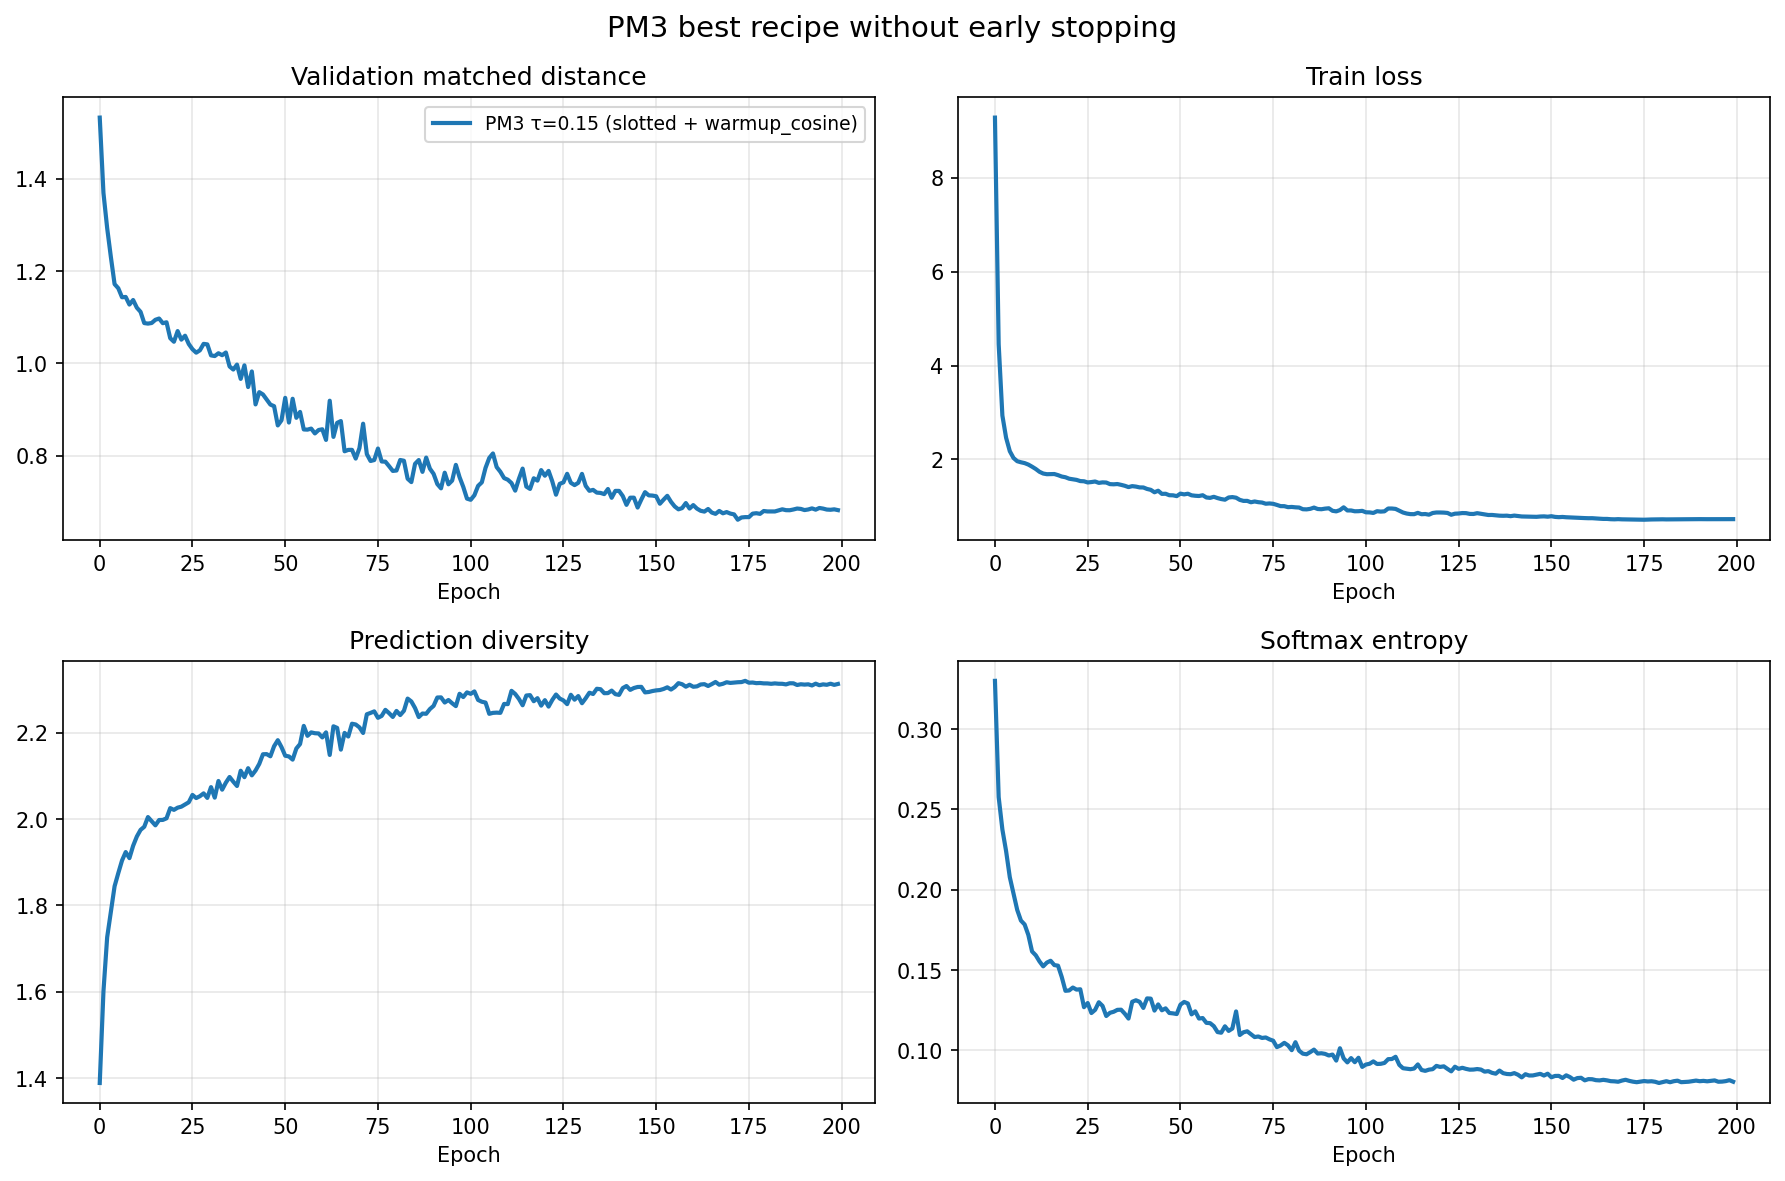
\includegraphics[width=\textwidth,height=0.63\textheight,keepaspectratio]{pm3_best_recipe_no_earlystop_monitoring.png}

\vspace{0.3em}
\footnotesize
\begin{itemize}
  \item Early stopping was a real confounder: best dist improves from $0.7039$ to $0.6607$ without truncation.
  \item But even the full 200-epoch rerun still lags the best single-factor PM3 variants.
  \item Conclusion: early stopping hurt this run, but it is not the whole explanation.
\end{itemize}
\end{frame}

\begin{frame}{PM3 Recipe Comparison}
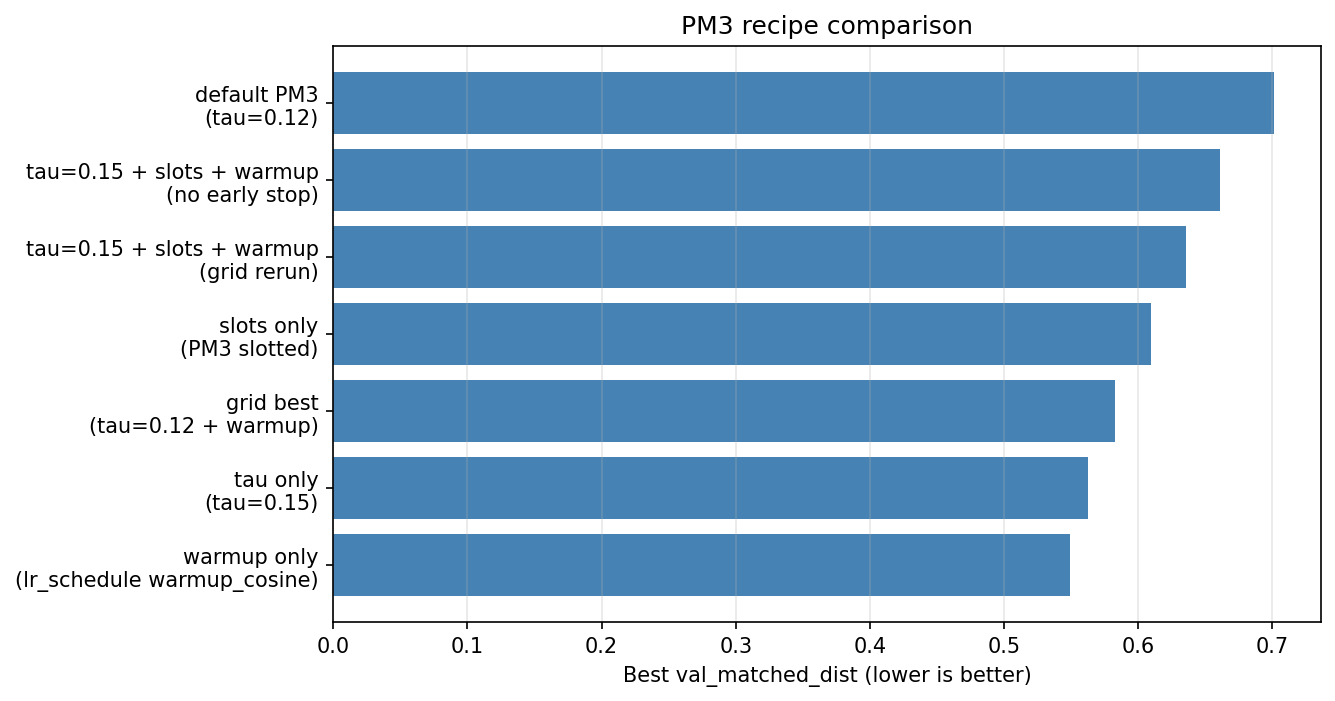
\includegraphics[width=\textwidth,height=0.63\textheight,keepaspectratio]{pm3_recipe_comparison.png}

\vspace{0.3em}
\footnotesize
\begin{itemize}
  \item The best PM3 points are warmup-only ($0.5495$), tau-only ($0.5625$), and the grid winner ($0.5828$).
  \item The full $\tau=0.15$ + slots + warmup recipe is worse in both the grid rerun ($0.6353$) and the no-early-stop rerun ($0.6607$).
  \item This is strong evidence that the PM3 gains are non-additive.
\end{itemize}
\end{frame}

\begin{frame}{2x2x2 PM3 Grid}
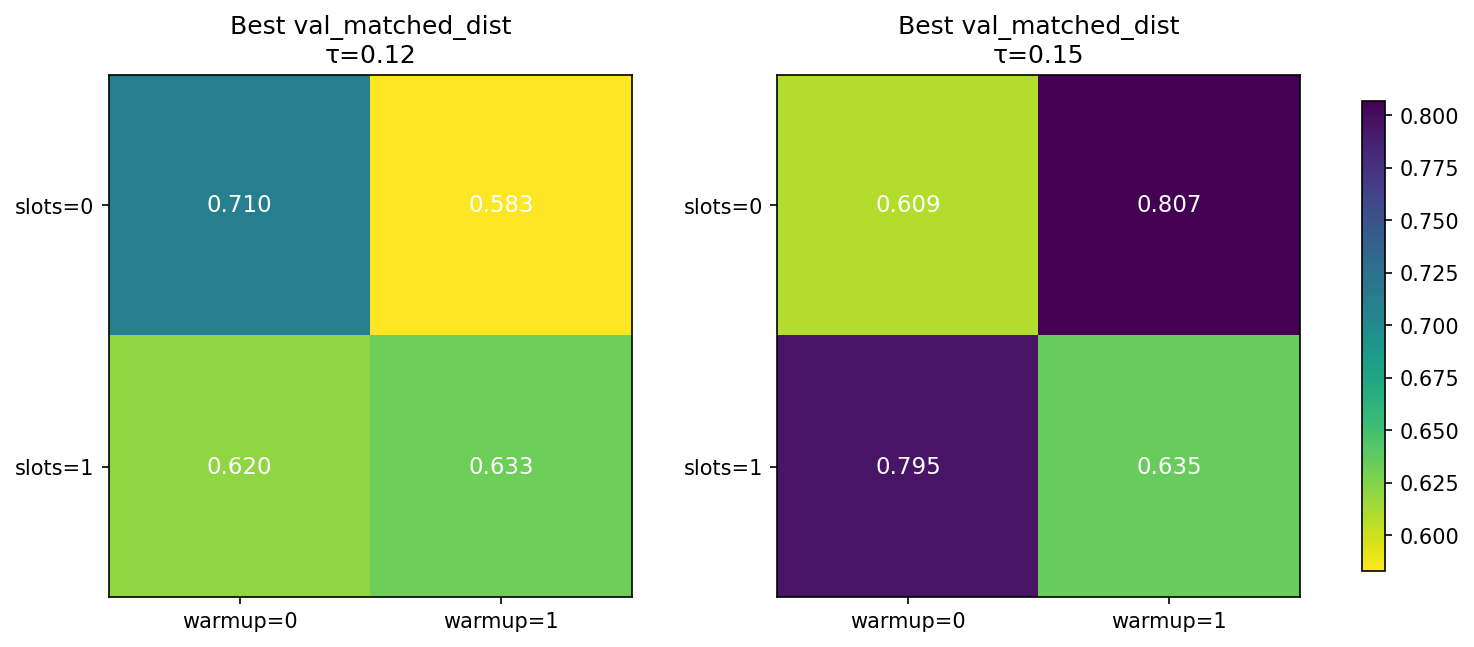
\includegraphics[width=\textwidth,height=0.63\textheight,keepaspectratio]{pm3_grid_best_dist.png}

\vspace{0.3em}
\footnotesize
\begin{itemize}
  \item Best clean PM3 recipe in the grid: $\tau=0.12$ + warmup + standard decoder at $0.5828$.
  \item Slots help at $\tau=0.12$ without warmup ($0.6199$), but stop helping once warmup is added.
  \item At $\tau=0.15$, warmup actually hurts the standard decoder badly ($0.6090 \rightarrow 0.8069$).
\end{itemize}
\end{frame}

\begin{frame}{Why The Combined Recipe Is Not Additive}
\small
\begin{itemize}
  \item Slots likely help PM3 by breaking symmetry when the decoder is otherwise too exchangeable.
  \item warmup\_cosine also smooths optimization, and a hotter $\tau$ softens responsibility assignment.
  \item Combining all three can over-smooth the PM3 objective: coverage is maintained, but the push toward sharp, consistent assignments weakens.
  \item Hungarian benefits from the same architectural and schedule improvements because its assignment step stays discrete.
  \item The gap between the grid rerun and the separate no-early-stop rerun also suggests narrower, more brittle optimization basins for the combined PM3 recipe.
\end{itemize}
\end{frame}

\begin{frame}{Computational Cost Comparison}
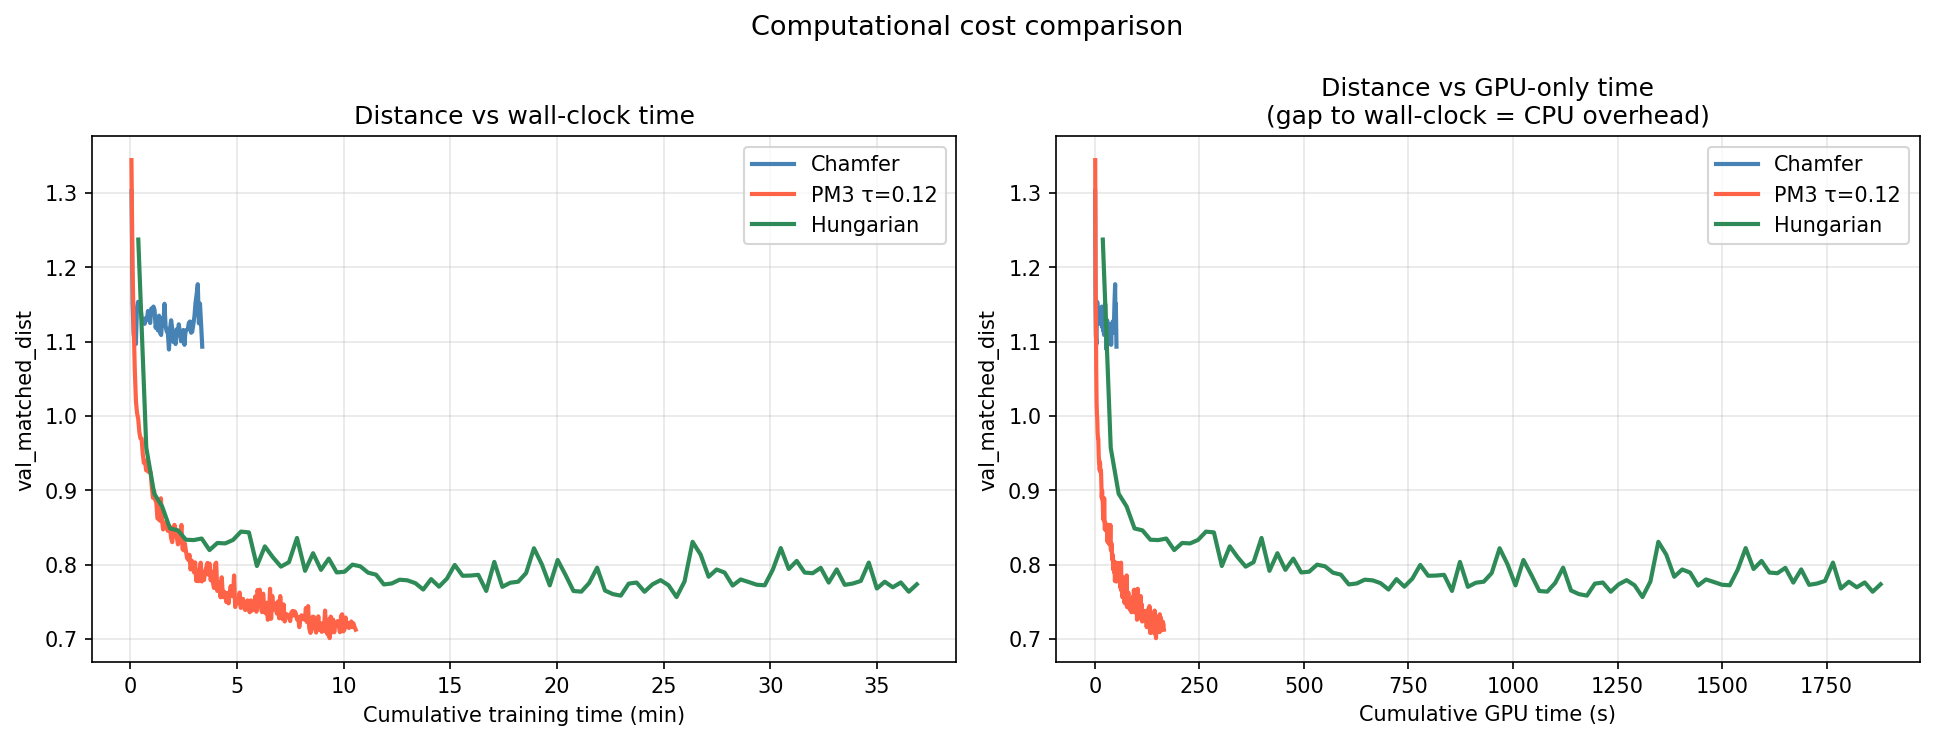
\includegraphics[width=\textwidth,height=0.60\textheight,keepaspectratio]{cost_comparison.png}

\vspace{0.3em}
\footnotesize
\begin{itemize}
  \item PM3 reaches $0.80$ in 2.82 min; Hungarian reaches it in 5.93 min; Chamfer never does.
  \item PM3 and Chamfer both run around 6 ms/batch; Hungarian is about 139 ms/batch.
  \item Hungarian can still reach a better final distance than default PM3 only when given the stronger combined recipe.
\end{itemize}
\end{frame}

\begin{frame}{Benchmark Validity}
\small
\begin{itemize}
  \item This CLEVR study was very effective for parameter search and mechanism analysis.
  \item It is not the final community benchmark story: the current task is a state-denoising proxy with matched-distance evaluation, not the most popular image-to-set benchmark in the loss/matching literature.
  \item For a mainstream `$X \rightarrow \mathrm{set}$` benchmark with a rich assignment literature, COCO detection in a DETR-style setup is the right next target.
  \item So the correct framing is:
  \begin{itemize}
    \item CLEVR = fast studybed to find promising PM3 settings
    \item COCO DETR = benchmark to test whether PM3-like matching holds up in a widely studied setting
  \end{itemize}
\end{itemize}
\end{frame}

\begin{frame}{Confirmed Next Steps}
\small
\begin{itemize}
  \item Keep the CLEVR study outputs, slides, scripts, and utilities in a dedicated study area instead of scattered repo roots.
  \item Carry forward two PM3 candidates: the strongest clean grid point and the best single-factor PM3 wins.
  \item Bootstrap a dedicated COCO DETR benchmark area with:
  \begin{itemize}
    \item a canonical Hungarian DETR baseline
    \item a PM3-like soft matching variant on the same class + box cost matrix
    \item reduced-data smoke tests before full COCO training
  \end{itemize}
  \item Compare AP, convergence speed, duplicate behavior, and training stability before making broader claims.
\end{itemize}
\end{frame}

\end{document}
